\section{Results}\label{sec:results}

All numbers below come from \texttt{results/report\_main.json}, produced by
\texttt{scripts/run\_experiments.py} at the pinned commit, and are inserted into this document by
\texttt{paper/analysis.py}. The evaluated grid is \NumPairs{} task--fault pairs
(\NumHarmful{} harmful) over \NumEpisodes{} episodes.

\subsection{Detection is easier than repair}

\begin{table}[t]
\centering\small
\caption{Failure detection at the step level. Precision, recall and F1 are
computed on \emph{step-level} labels (is a fault active at this step?), so a
detector that fires every step scores high recall and low precision. AUC is
threshold-free. \emph{Type} is the accuracy of the predicted class among
positive steps. \emph{Instrumented} exposes harness telemetry flags;
\emph{blackbox} hides them, leaving only error codes, payloads, version
counters and timing.}
\label{tab:detection}
\begin{tabular}{@{}llcccccc@{}}
\toprule
Detector & Monitor & Prec. & Rec. & F1 & AUC & Type & Steps \\
\midrule
Rules & instrumented & 66.9 & 41.9 & 51.5 & 0.772 & 34.6 & 24,175 \\
Rules & blackbox & 86.7 & 32.0 & 46.7 & 0.787 & 22.1 & 1,094 \\
Supervised & instrumented & 48.8 & 86.2 & 62.3 & 0.762 & 51.6 & 11,193 \\
Supervised & blackbox & 46.0 & 81.0 & 58.7 & 0.750 & 39.9 & 1,060 \\
\bottomrule
\end{tabular}
\end{table}


The rule detector reaches AUC \AucRules{} (F1 \RulesFone\%, precision \RulesPrecision\%,
recall \RulesRecall\%), and the supervised detector is comparable (AUC \AucSupervised{}, F1
\SupFone\%, type accuracy \SupTypeAcc\% vs \RulesTypeAcc\% for rules). With cluster-bootstrap
intervals the rule monitor's step-level F1 is \RulesFone\% [\RulesFoneLo, \RulesFoneHi] and AUC
\AucRules{} [\AucRulesLo, \AucRulesHi] over \DetectionClusters{} templates
(Table~\ref{tab:detection_ci}); the intervals are wide because whole templates are resampled,
which is the honest resolution of a grid with three of them. Two things are worth
separating. First, aggregate AUC is respectable but \emph{class} accuracy is only around
35--50\%, i.e.\ the monitor usually knows that something is wrong and often does not know what.
Since the recovery policy is indexed by class, that confusion is expensive downstream: a stale read
labelled as a planning error triggers a replan that does not re-read, and the failure survives the
repair. Second, hiding the telemetry flags (blackbox) barely dents AUC (\AucRulesBlackbox{} for
rules, versus \AucRules{} instrumented; Fig.~\ref{fig:gap}) but does cost detection \emph{coverage}
in the recovery loop, because the latent classes lose their most reliable evidence. That cost is
large: with the identical rule detector and rule-based policy, a black-box monitor recovers
\BlackboxRecRules\% [\BlackboxRecRulesLo{}, \BlackboxRecRulesHi{}] of harmful faults, against
\RecRules\% when the runtime exposes its own staleness, conflict and message-loss telemetry. In
other words the ordering of a leaderboard entry is stable across regimes, but the absolute
reliability a deployment can expect is not---which is why the protocol requires both columns.

\begin{figure}[t]
\centering
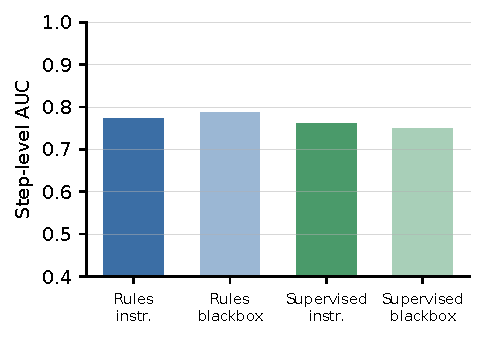
\includegraphics[width=0.62\linewidth]{figures/fig_gap.pdf}
\caption{Detectability gap. Step-level AUC is nearly unchanged when harness telemetry is hidden, but
type identification degrades---a monitor can see that something is wrong from error strings and
version counters without being able to say what it is.}
\label{fig:gap}
\end{figure}

Signal ablation (Table~\ref{tab:ablation}) shows error codes carry the most mass (removing them drops
event detection from 88\% to 64\%), with policy conformance and version staleness next at 74\%. A
monitor built purely on error codes is therefore not viable: the classes that dominate the harmful
set are not error-code failures.

\begin{table}[t]
\centering\small
\caption{Signal ablation for the rule-based detector: each row removes one
feature family and reports event-level detection rate. Error codes carry the most
mass; removing policy conformance or version/staleness loses a comparable share,
which is why a purely error-driven monitor is insufficient.}
\label{tab:ablation}
\begin{adjustbox}{max width=\textwidth}
\begin{tabular}{@{}lc@{}}
\toprule
Feature set & Detected (\%) \\
\midrule
full & 88.0 \\
$-$ error\_codes & 64.0 \\
$-$ version\_staleness & 74.0 \\
$-$ conflict & 80.0 \\
$-$ communication & 88.0 \\
$-$ progress & 88.0 \\
$-$ policy\_conformance & 74.0 \\
\bottomrule
\end{tabular}
\end{adjustbox}
\end{table}


\subsection{Recovery is class-dependent, and not in the order you would guess}

\begin{table}[t]
\centering\small
\caption{Recovery rate (\%) conditional on failure class. \emph{Det.} is the
rule-based detector's event recall for that class. Unrecoverable external errors
are reported as attempted repairs: the correct behaviour is containment, which is
scored separately (Sec.~\ref{sec:results}).}
\label{tab:bytype}
\begin{adjustbox}{max width=\textwidth}
\begin{tabular}{@{}lcccccc@{}}
\toprule
Failure class & No rec. & Retry & Rule & Model & Det. & $n$ \\
\midrule
invalid\_arguments & 0.0 & 0.0 & 95.9 & 73.4 & 100.0 & 169 \\
stale\_state & 0.0 & 0.0 & 76.3 & 68.4 & 86.8 & 76 \\
contradictory\_evidence & 0.0 & 0.0 & 96.2 & 96.2 & 100.0 & 158 \\
planning\_error & 0.0 & 0.0 & 40.9 & 41.8 & 80.0 & 110 \\
communication\_failure & 0.0 & 0.0 & 82.2 & 82.2 & 100.0 & 45 \\
objective\_drift & 0.0 & 0.0 & 52.2 & 23.1 & 97.8 & 134 \\
unrecoverable\_external\_error & 0.0 & 0.0 & 0.0 & 0.0 & 100.0 & 169 \\
\midrule
All & 0.0 & 0.0 & 60.9 & 51.3 & 95.9 & -- \\
\bottomrule
\end{tabular}
\end{adjustbox}
\end{table}


\begin{figure}[t]
\centering
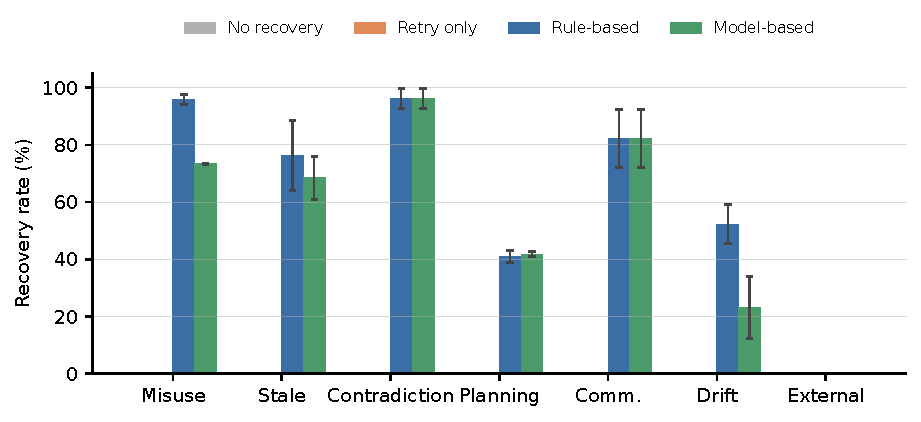
\includegraphics[width=\linewidth]{figures/fig_bytype.pdf}
\caption{Recovery by failure class with 95\% cluster-bootstrap intervals. Retries never help, and
the two classes that require an internal model of the task---planning error and objective
drift---are where recovery collapses.}
\label{fig:bytype}
\end{figure}

Table~\ref{tab:bytype} and Fig.~\ref{fig:bytype} are the core result. The ordering is not the
intuitive one. \emph{Contradictory evidence} is repaired 96\% of the time and \emph{misuse}
(mis-specified arguments) 96\%, despite the former being a ``latent'' class: both have a decisive,
cheap, local operator (re-read the authoritative source; re-derive the arguments). \emph{Planning
error} is repaired only 41\% and \emph{objective drift} 52\%, and those are the two classes whose
repair requires reconstructing what the task was supposed to accomplish. A replan that does not
recover the original objective simply produces a different wrong plan. This ordering is a
property of the repair operators, not of which selector chose them: the canonical mapping and
the learned ranker differ significantly after Holm correction in only
\HolmClassSignificant{} of \HolmClassTests{} classes---misuse and objective drift---and in both
the canonical mapping wins episode for episode (Table~\ref{tab:appendix_tests_class}). Where a
class has a cheap local operator, every selector finds it; where it does not, no selector does.

Two mechanical observations matter for anyone building on this. First, \emph{retry never works}:
retry-only recovers \RecRetry\% while spending more tool calls than the rule-based policy, because
retrying a deterministic tool reproduces the same failure and burns the budget. Second,
\emph{unrecoverable external errors are correctly contained but never recovered}, which is the right
answer; a policy that reports recovery on this class is either lying or was scored from self-report.

We also observe a systematic misattribution: in the accounting family the \texttt{close\_period}
precondition turns a silent objective-drift injection into a precondition error, so the monitor
labels it \emph{planning error} and applies the wrong operator. This is not a bug we patched away;
it is the phenomenon that makes drift hard---the surface signal points at the wrong class---and it is
part of why drift recovery sits at 52\%.

\subsection{Timing predicts recovery}

Detection \emph{speed} is not merely a diagnostic nicety. Splitting rule-based episodes by whether
the fault was detected at or before the injection step (i.e.\ before it could propagate) gives
\EarlyRec\% recovery over \EarlyN{} episodes versus \LateRec\% over \LateN{} late detections---a
\EarlyGap{} point gap. We report it as an association rather than a controlled effect, since
early-detectable faults are also the faults with the most visible signatures.

\begin{figure}[t]
\centering
\begin{subfigure}{0.48\linewidth}
\centering
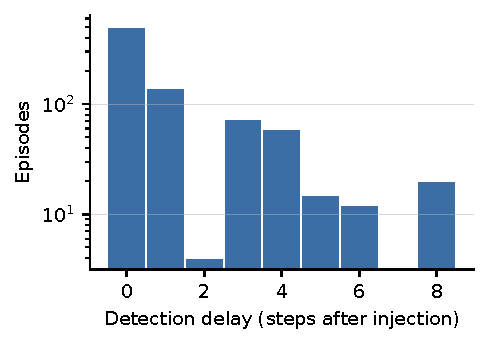
\includegraphics[width=\linewidth]{figures/fig_ttd.pdf}
\caption{Detection delay (rule-based).}
\end{subfigure}\hfill
\begin{subfigure}{0.48\linewidth}
\centering
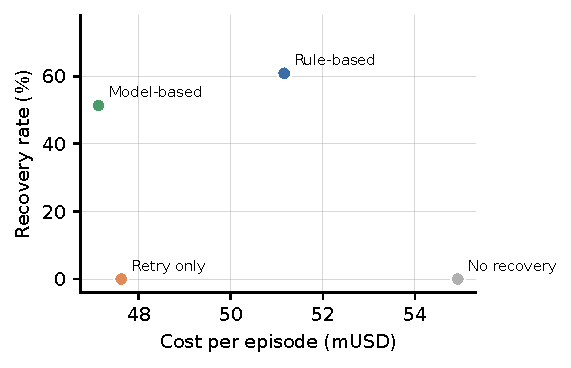
\includegraphics[width=\linewidth]{figures/fig_cost.pdf}
\caption{Cost vs.\ recovery.}
\end{subfigure}
\caption{Left: most detections land on the injection step, with a tail out to several steps. Right:
the cost-recovery frontier; the rule-based policy dominates on both axes, and ``no recovery'' is not
cheap because failed episodes run longer.}
\label{fig:ttd}
\end{figure}

\subsection{The learned ranker does not beat the canonical mapping}

\begin{table}[t]
\centering\small
\caption{Recovery performance by policy on the harmful-fault set
($n=\NumHarmful$ task--fault pairs per policy). Intervals are 95\% cluster
bootstrap over task templates. \emph{Tokens} is total model+tool tokens per
episode; \emph{USD} uses the fixed price sheet (Sec.~\ref{sec:cost}).}
\label{tab:main}
\begin{tabular}{@{}lccccccc@{}}
\toprule
Policy & Recovery \% [95\% CI] & Single & Multi & Detected \% & Calls & Tokens & USD \\
\midrule
No recovery & 0.0 [0.0, 0.0] & 0.0 & 0.0 & 0.0 & 14.34 & 17432 & 0.0549 \\
Retry only & 0.0 [0.0, 0.0] & 0.0 & 0.0 & 95.9 & 12.50 & 15134 & 0.0476 \\
Rule-based & 60.9 [57.9, 65.3] & 68.2 & 46.0 & 95.9 & 13.76 & 16074 & 0.0512 \\
Model-based & 51.3 [50.5, 51.7] & 59.4 & 35.1 & 99.4 & 13.00 & 14711 & 0.0471 \\
\bottomrule
\end{tabular}
\end{table}


Table~\ref{tab:main} is the headline comparison. No recovery: \RecNoRecovery\%. Retry only:
\RecRetry\%. Rule-based: \RecRules\%. Model-based: \RecModel\%. The learned ranker is a genuine
attempt---per-operator value models, calibrated features, a real candidate set---and it lands
\emph{below} the hand-written mapping. The diagnosis is off-policy confounding: the ranker only ever
sees the outcome of operators the rule-based policy chose, so for any state where the canonical
operator failed it has no counterfactual to learn from, and its containment head (which has the
fewest logged executions) fires on states where repair would have worked. We report this as a
boundary result: \emph{learning when to repair is not the bottleneck; learning what to repair
requires exploration the logged data does not contain.} The gap is not sampling noise: an exact
McNemar test on the \StatsPairs{} paired episodes rejects equality of the two policies
($b=\RuleVsModelB$ pairs recovered only by the canonical mapping, $c=\RuleVsModelC$ only by the
ranker, $p=\RuleVsModelP$), and it survives Holm correction over the \HolmPolicyTests{} policy
pairs ($p_{\text{Holm}}=\RuleVsModelPHolm$; Table~\ref{tab:appendix_tests_policy}).

\subsection{An LLM controller does not close the gap either}

\begin{table}[t]
\centering\small
\caption{Operator selection by a language model versus the canonical mapping, on identical
harmful pairs (\LLMPairs\ sampled harmful pairs, local model \texttt{\LLMModel}, detector held fixed at the rule monitor). The detector, the recovery programs and the grader are shared,
so the difference is attributable to which operator is applied.}
\label{tab:llm}
\begin{adjustbox}{max width=\textwidth}
\begin{tabular}{@{}lcccc@{}}
\toprule
Failure class & $n$ & Rule-based & LLM & $\Delta$ (pp) \\
\midrule
invalid\_arguments & 44 & 95.5 & 95.5 & +0.0 \\
stale\_state & 30 & 80.0 & 80.0 & +0.0 \\
contradictory\_evidence & 44 & 95.5 & 0.0 & -95.5 \\
planning\_error & 30 & 33.3 & 0.0 & -33.3 \\
communication\_failure & 11 & 81.8 & 0.0 & -81.8 \\
objective\_drift & 41 & 46.3 & 0.0 & -46.3 \\
unrecoverable\_external\_error & 40 & 0.0 & 0.0 & +0.0 \\
All & 240 & 60.8 & 27.5 & +33.3 \\
\bottomrule
\end{tabular}
\end{adjustbox}
\end{table}


The learned ranker is not the only selector we tried. To test whether the shortfall is a property of
our small model class rather than of the problem, we replace \emph{only} the operator-selection step
with a locally served 7B instruction model (\texttt{\LLMModel}, temperature 0, JSON-constrained
output). The detector, the nine recovery programs, the environments and the grader are unchanged, so
the comparison isolates the choice of operator; the prompt carries the detector's posterior and the
monitor feature vector plus the operator menu, and never the injected fault, its injection step, the
expected state or the grader's verdict. Replies are cached by prompt hash, so the arm replays exactly.
On \LLMPairs harmful pairs stratified by class \emph{and} family, the same pairs are replayed with
the canonical mapping: the LLM recovers \LLMRecovery\% against \LLMRuleRecovery\% for the rules, a
paired lead of \LLMPairedDelta{} points [\LLMPairedLo{}, \LLMPairedHi{}]. The interval is wide because
the cluster bootstrap resamples three templates; the point difference is not. An exact McNemar
test on the same \LLMPairs{} pairs rejects equality of the two selectors: the canonical mapping
recovers $b=\LLMMcNemarB$ pairs the LLM misses, and the LLM recovers $c=\LLMMcNemarC$ that the
mapping does not, $p=\LLMMcNemarP$. That test is pre-specified on its own 240-pair sample, so it
enters no Holm family (App.~\ref{app:tests}).

The pattern of failure is more informative than the aggregate. Where the class is \emph{surface} and
its name names its repair, the model reproduces the canonical mapping decision for decision---misuse
at \LLMMisuse\% (rules \LLMRuleMisuse\%), stale state at \LLMStale\% (rules \LLMRuleStale\%)---because
the menu entry (\texttt{revalidate\_args}, \texttt{refresh\_state}) is the obvious reading of the
alarm. Where the class is \emph{latent}---contradictory evidence, planning error, objective
drift---it falls back to \texttt{retry} (\LLMRetryPct\% of its \LLMDecisions{} decisions), which
repairs none of them, and on the unrecoverable class it retries instead of halting, containing
\LLMContainment\% of outages against \LLMRuleContainment\% for the rules. Reading a mapping that is
written down is within reach of a small model; \emph{inferring} one from evidence is not. The
\LLMCalls{} billed model calls cost nothing beyond the local server, so this is a capability result,
not a budget artefact.

\subsection{Held-out generalisation}

\begin{table}[t]
\centering\small
\caption{Held-out generalisation. \emph{test\_id} uses a seen task template
with an unseen environment configuration (higher concurrency); \emph{test\_ood}
uses an entirely held-out template. Detectors and rankers are fit on
\emph{train} only. Recovery rate (\%) with episode count in parentheses.}
\label{tab:split}
\begin{adjustbox}{max width=\textwidth}
\begin{tabular}{@{}lcccc@{}}
\toprule
Policy & Train & Dev & Test (ID) & Test (OOD) \\
\midrule
Rule-based & 60.7 (351) & 67.9 (109) & 62.4 (109) & 57.9 (292) \\
Model-based & 49.3 (351) & 52.3 (109) & 56.0 (109) & 51.7 (292) \\
\bottomrule
\end{tabular}
\end{adjustbox}
\end{table}


Generalisation is reassuringly flat (Table~\ref{tab:split}): the rule-based policy recovers 62.4\% on
the unseen configuration and 57.9\% on the unseen template, against 60.7\% on train, and the
model-based policy shows the same mild degradation. The detector and ranker never saw the held-out
template, so the taxonomy-based rules are doing real work rather than memorising schedules. The OOD
drop is concentrated in the migration family, where the held-out template adds a reconciliation
branch that the canonical operator program handles less directly.

\subsection{Single-agent versus multi-agent}

There is a consistent multi-agent penalty: \MultiRecovery\% recovery on multi-agent episodes versus
\SingleRecovery\% on single-agent episodes over the same fault classes. Part of this is structural
(multi-agent tasks have longer horizons and more state), but a specific mechanism is visible in the
coordination slice: \emph{communication failure} is repaired 82\% of the time by the rule-based
policy---the highest of any class---\emph{when} the bus can be re-synchronised, because the operator
(\texttt{resync\_message}) restores the receiving role's belief directly. Without it the failure is
invisible to the receiving agent: its belief is simply wrong, and no amount of re-reading its own
tools fixes a message it never got. Communication is therefore the class where multi-agent recovery
is qualitatively different from single-agent recovery rather than merely harder.

\subsection{The self-report gap}

Agents claim success in \ClaimedPct\% of evaluated episodes and are verified successful in
\VerifiedPct\%. \FalseClaimPct\% of episodes with a success claim failed the state check
(\FalseClaimN{} episodes). The gap is not uniform: it is largest in the migration family, where
``copied everything I was shown'' is true and ``everything was copied'' is false---a silent lost
update the agent has no way to observe. Any evaluator that reads the transcript, or asks the agent
whether it succeeded, would have scored those runs as wins. This is the single strongest argument for
state-verified scoring in this benchmark and we treat it as a finding, not a footnote.

\subsection{Cost}

\begin{table}[t]
\centering\small
\caption{Cost-aware outcomes under the fixed price sheet. \emph{USD/episode}
is the mean over all evaluated episodes; \emph{USD/recovered} is the total spend
divided by the number of recovered episodes, i.e.\ the amortised price of a
successful repair; \emph{USD/failed} is the mean spend on episodes that still
failed. Recovery is never free: detection and repair consume steps, tokens and
tool calls.}
\label{tab:cost}
\begin{adjustbox}{max width=\textwidth}
\begin{tabular}{@{}lccccc@{}}
\toprule
Policy & USD/episode & USD/recovered & USD/failed & Latency (ms) & Recovery \% \\
\midrule
No recovery & 0.0549 & -- & 0.0549 & 4927 & 0.0 \\
Retry only & 0.0476 & -- & 0.0476 & 4334 & 0.0 \\
Rule-based & 0.0512 & 0.0841 & 0.0341 & 4699 & 60.9 \\
Model-based & 0.0471 & 0.0918 & 0.0358 & 4452 & 51.3 \\
\bottomrule
\end{tabular}
\end{adjustbox}
\end{table}


Recovery is not free and ``no recovery'' is not cheap. Because failed episodes run to the end of the
procedure and retry, the no-recovery baseline spends \emph{more} than the rule-based policy in total
(Table~\ref{tab:cost}); repair truncates doom loops. The amortised view (USD per recovered episode)
is the fair comparison for a deployment: it prices the failures that were never repaired into the
cost of the ones that were. On that metric the rule-based policy is the only policy whose spend buys
recovery rather than activity.

\begin{figure}[t]
\centering
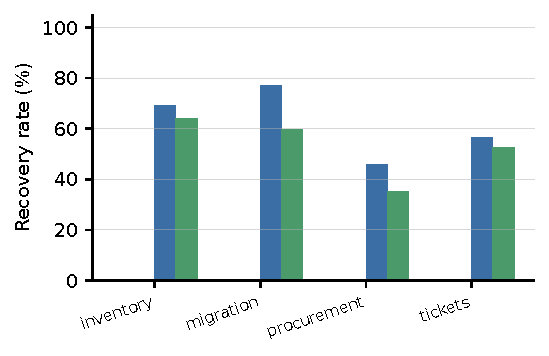
\includegraphics[width=0.6\linewidth]{figures/fig_family.pdf}
\caption{Recovery by environment family. The accounting family is hardest for every policy, and the
gap between rule-based and no-recovery is largest where state is auditable.}
\label{fig:family}
\end{figure}

\subsection{Provenance shift and long horizons}

\begin{table}[t]
\centering\small
\caption{Provenance shift: detections on faults produced by the agent's own
competence model rather than by the injection machinery ($n=\NaturalN$ episodes;
the rule-based policy and detector are used unchanged). Detected
\NaturalDetected\%, recovered \NaturalRecovery\%, class agreement
\NaturalAgreement\%.}
\label{tab:natural}
\begin{tabular}{@{}lc@{}}
\toprule
Agent-side failure class & Episodes \\
\midrule
invalid\_arguments & 12 \\
objective\_drift & 11 \\
planning\_error & 16 \\
\bottomrule
\end{tabular}
\end{table}


When failures are produced by the agent's own competence model instead of the injection machinery
(Table~\ref{tab:natural}), the unchanged rule detector finds \NaturalDetected\% of them and the
rule-based policy recovers \NaturalRecovery\%, with \NaturalAgreement\% agreement between detected
and true class. Event recall is lower than on injected faults---natural faults often have quieter
signatures---but conditional recovery is \emph{higher}, because natural faults tend to be local. The
taxonomy transfers; the operating point does not, which is exactly why a leaderboard must report
both.

\begin{table}[t]
\centering\small
\caption{Long-horizon slice (2--3$\times$ the steps of the main grid, with fully
observable state and success criteria). Recovery rate (\%) with episode count,
mean time-to-detection in steps, and mean tool calls.}
\label{tab:long}
\begin{tabular}{@{}lcccc@{}}
\toprule
Family & No recovery & Rule-based & TTD & Calls \\
\midrule
inventory & 0.0 (19) & 68.4 (19) & 1.21 & 22.3 \\
migration & 0.0 (16) & 75.0 (16) & 0.75 & 29.8 \\
procurement & 0.0 (25) & 52.0 (25) & 2.42 & 13.4 \\
tickets & 22.2 (18) & 66.7 (18) & 0.29 & 18.4 \\
\bottomrule
\end{tabular}
\end{table}


Long-horizon tasks (Table~\ref{tab:long}) confirm the pattern at 2--3$\times$ the step count with
fully observable state: detection still lands within about a step of injection for rules, but
recovery rates fall and downstream impact grows, because there are more steps after the fault for the
damage to reach.
